\section{Måling av Masse}

\subsection{Innledning}

Andre eksperiment var delt inn i to forsøk, basert på forskjellige måter å måle et objekts masse. 
I det første forsøket (som jeg vil referere til som forsøk d), skulle vi bruke en fjærvekt til å måle elastisk deformasjon. Når det henger et objekt med masse $m$ i fjæren, vil gravitasjonskraften motvirkes av fjærkraften, gitt ved Hookes lov, ($F = k\cdot l$). Dette gir oss at Gravitasjonskraften er proporsjonal med fjærens utstrekning, og siden $G = mg$, der vi antar at $g$ er konstant, har vi at massen er proporsjonal med fjærens utstrekning, og at vi kan bruke fjæren til å anslå et objekts masse. \medskip

I det andre forsøket (videre referert til som forsøk e), skulle vi bruke en harmonisk oscillator til å anslå et objekts masse. Ved å se på hvordan oscillatorens svingetid endrer seg når masse legges til, kan vi anslå endringen i masse, og dermed hvor stor massen til objektet vi la til er. \medskip

Begge disse forsøkene introduserer konseptet kalibrering, altså hvordan man ved hjelp av kjente verdier kan sette opp måleinstrumenter til å måle ukjente verdier. I våre tilfeller bruker vi da altså objekter som vi vet massen til fra før, til å beregne masser vi ikke kjenner til fra før. Vi ønsker også, for begge forsøkene, å anslå et dynamisk område for måleinstrumentene. Dynamisk område er forholdet mellom den største og den minste verdien et instrument kan måle, og viser hvor godt et måleinstrument er til å måle verdier av forskjellige størrelsesordener.

\subsection{Material og Metoder}

Til forsøk d trengte vi en bladvekt til å måle deformasjon (se fig \ref{forsøk_d_fig}), et sett med kalibreringslodd med kjente masser (Våre hadde massene 1g, 10g, 100g, 500g, 1000g, og 2000g), hansker slik at vi ikke la igjen fingeravtrykk på kalibreringsloddene (dette ville ført til at loddene endret masse), og det store loddet med ukjent masse vi ønsker å måle (se fig \ref{forsøk_d_fig}).

\bigskip \hfil
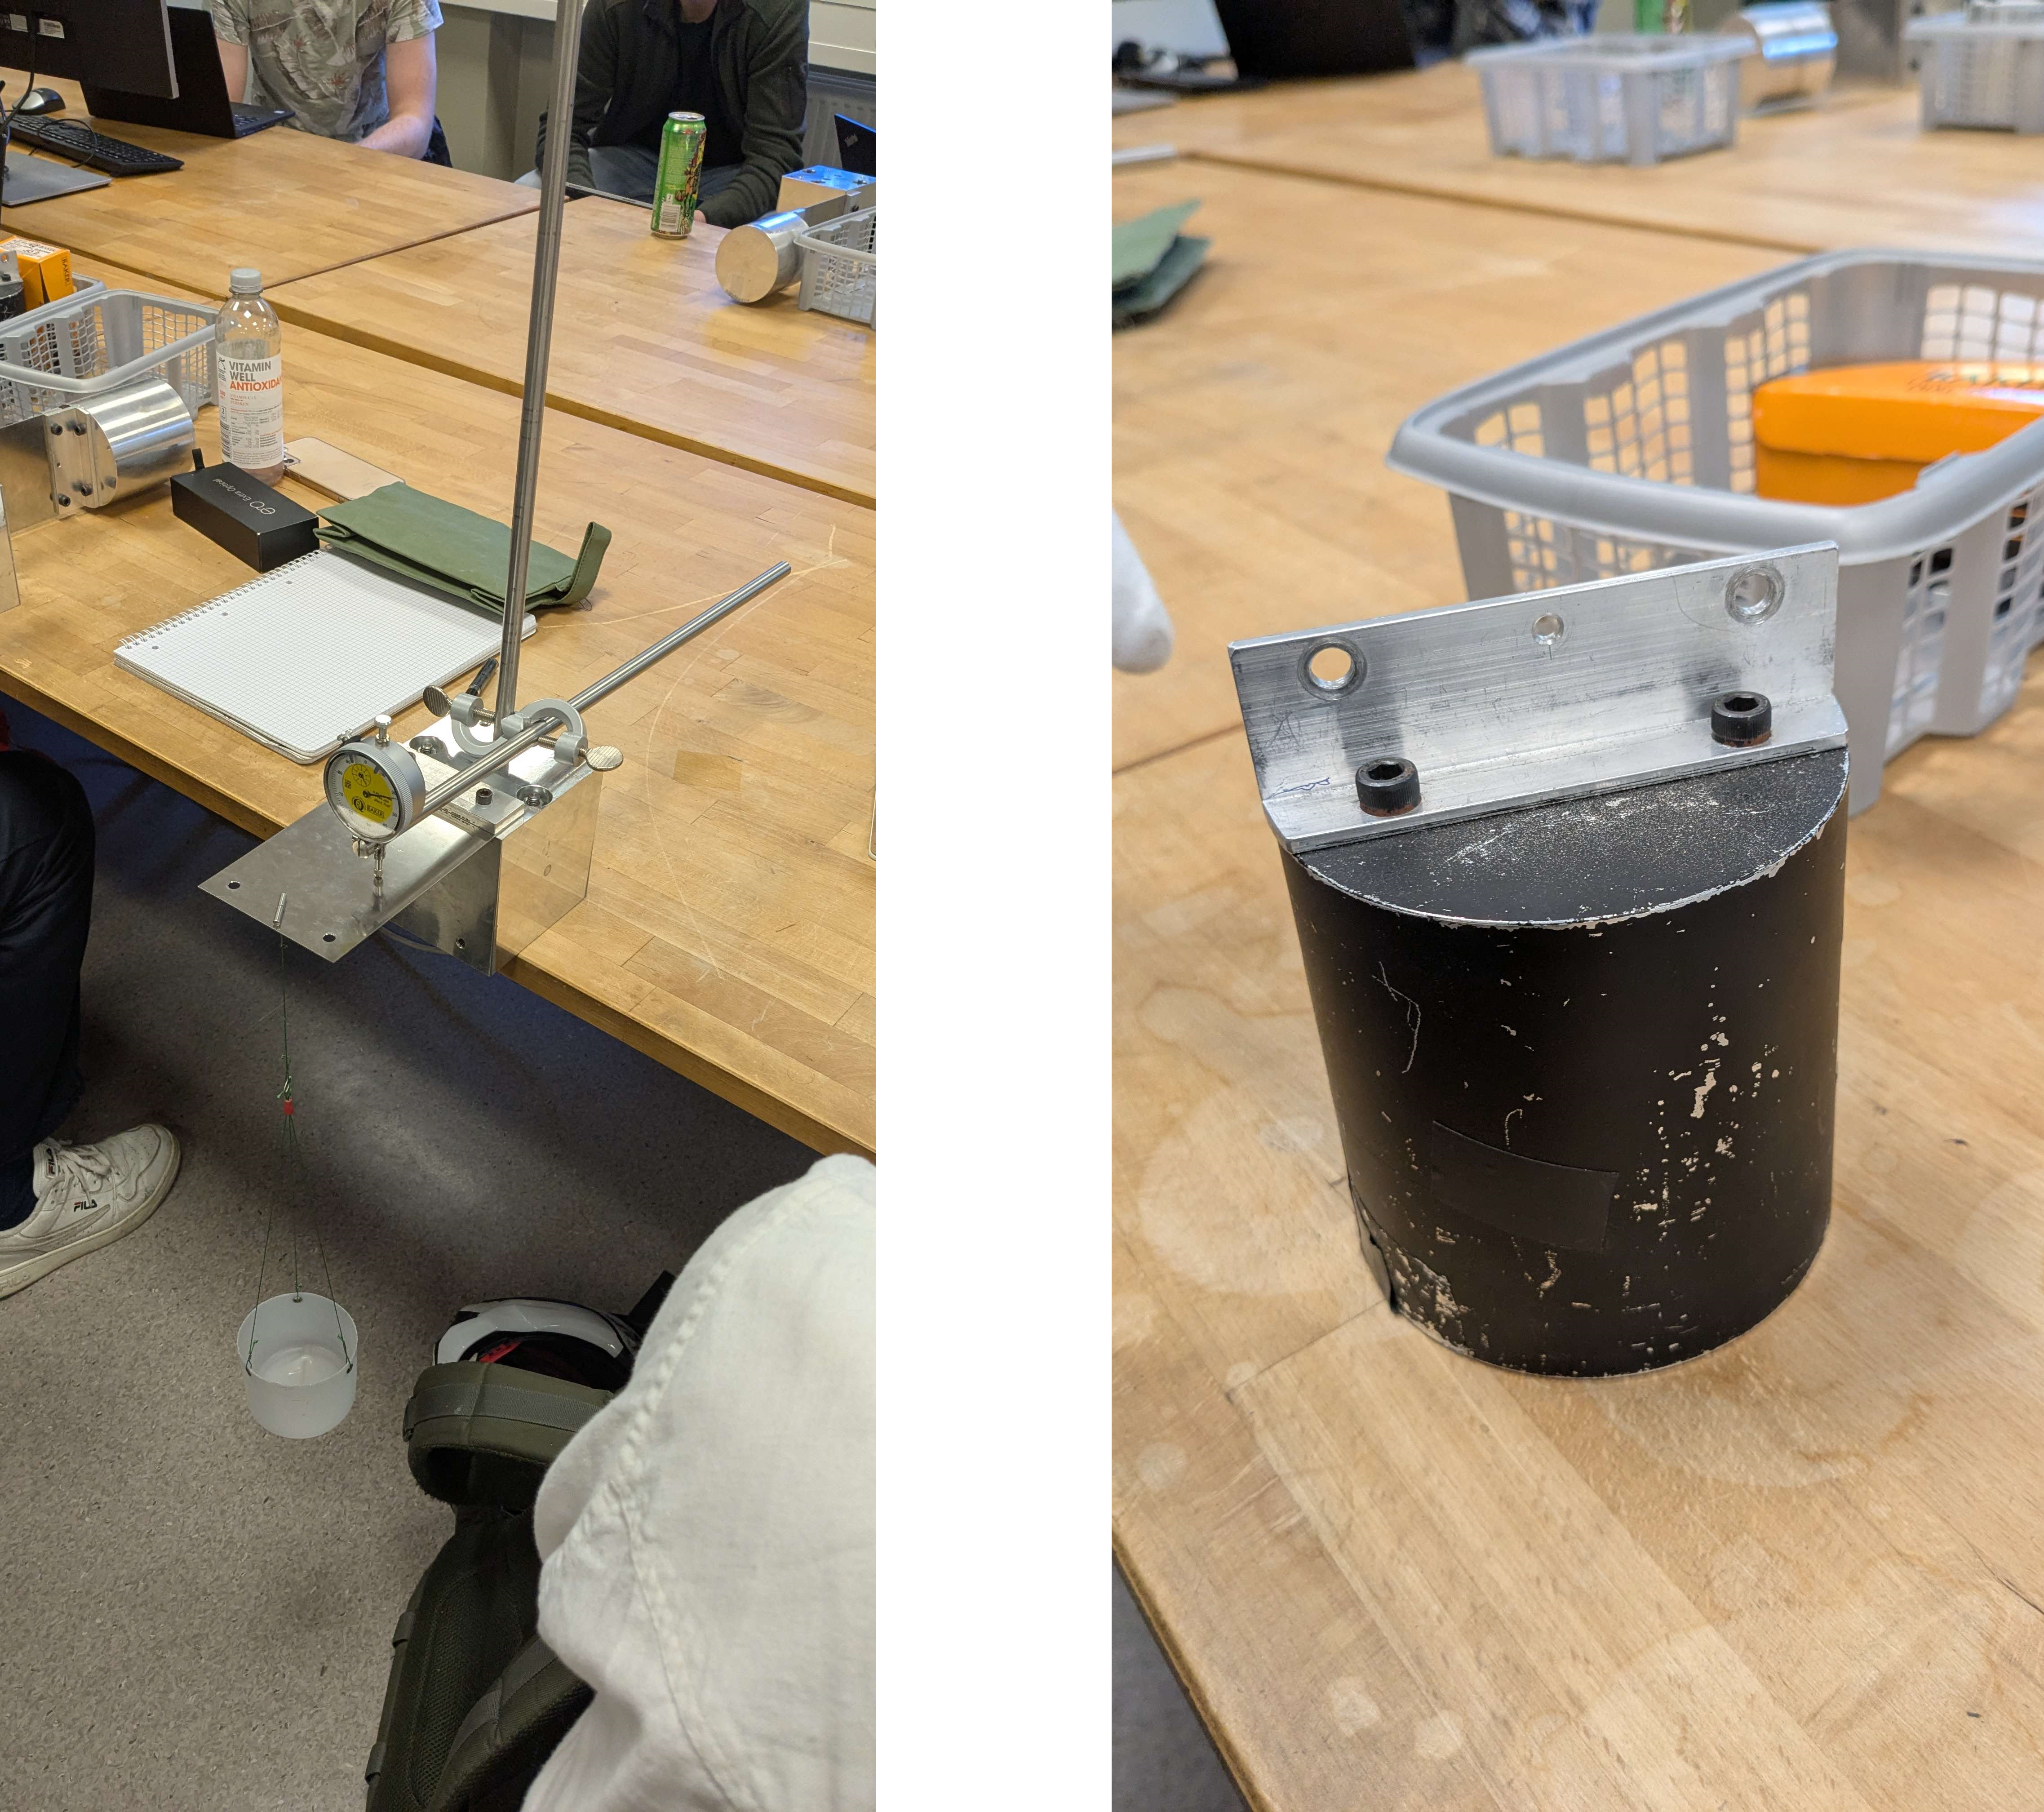
\includegraphics[scale = 0.07]{Figurer/Lab_Fig_d.png} 
\captionof{figure}{Bladvekt (venstre) og lodd med ukjent masse (høyre)} \label{forsøk_d_fig}
\par \bigskip

Vi begynte med å sjekke at loddet vi ønsket å måle var innenfor bladvektens rekkevidde. Vi plasserte loddet i kurven som var festet til bladet på vekten, og sjekket at dette ikke deformet bladet lenger enn det måleuret kunne måle.
Når vi hadde sjekket dette, begynte vi å kalibrere bladvekten. Vi leste av måleuret for mange kombinasjoner av kalibreringsloddene (Hvilke kombinasjoner er spesifisert i \nameref{Resultater_2}). \medskip

Så plottet vi en kalibreringskurve for bladvekten i python, og tilpasset en lineær regresjonsmodell til denne kurven, slik at vi kunne anslå massen til det ukjente loddet. Vi plottet også residualplott og prediksjonsintervall, for å finne usikkerheten i målingen. \bigskip

Til forsøk e trengte vi en harmonisk oscillator, vi brukte en pendel bygget opp av en bladfjær og et lodd (se fig \ref{forsøk_e_fig}). Vi trengte også en stoppeklokke (vi brukte mobiltelefoner), en digital-vekt, unbrakonøkkeler og binderser i varierende størrelser, og tape.

Først tok 20 målinger av pendelens svingetid, i 5 og 5 svingninger om gangen. Så målte vi massen til loddet vi brukte i forsøk d, for å estimere massen til loddet vårt. Vi brukte så følgende formel til å estimere fjærkonstanten.

\begin{align}
    T =2\pi\sqrt{m/k} \label{periodformula}
\end{align}

Så brukte vi samme formel, sammen med følgende formel for å estimere usikkerheten i massen $u_m$. Dette er da den minste endringen i masse vi kan måle.

\begin{align}
    u_f^2 = \left(\frac{\delta f}{\delta x} u_x\right)^2 + \left(\frac{\delta f}{\delta y} u_y\right)^2\label{gu}
\end{align}

Vi teipet sammen umbrakonøkkeler og binderser fram til de hadde masse ca. lik $u_m$, og festet dette til pendelen (se fig \ref{forsøk_e_fig}). Vi målte så pendelens svingetid igjen.

\bigskip \hfil
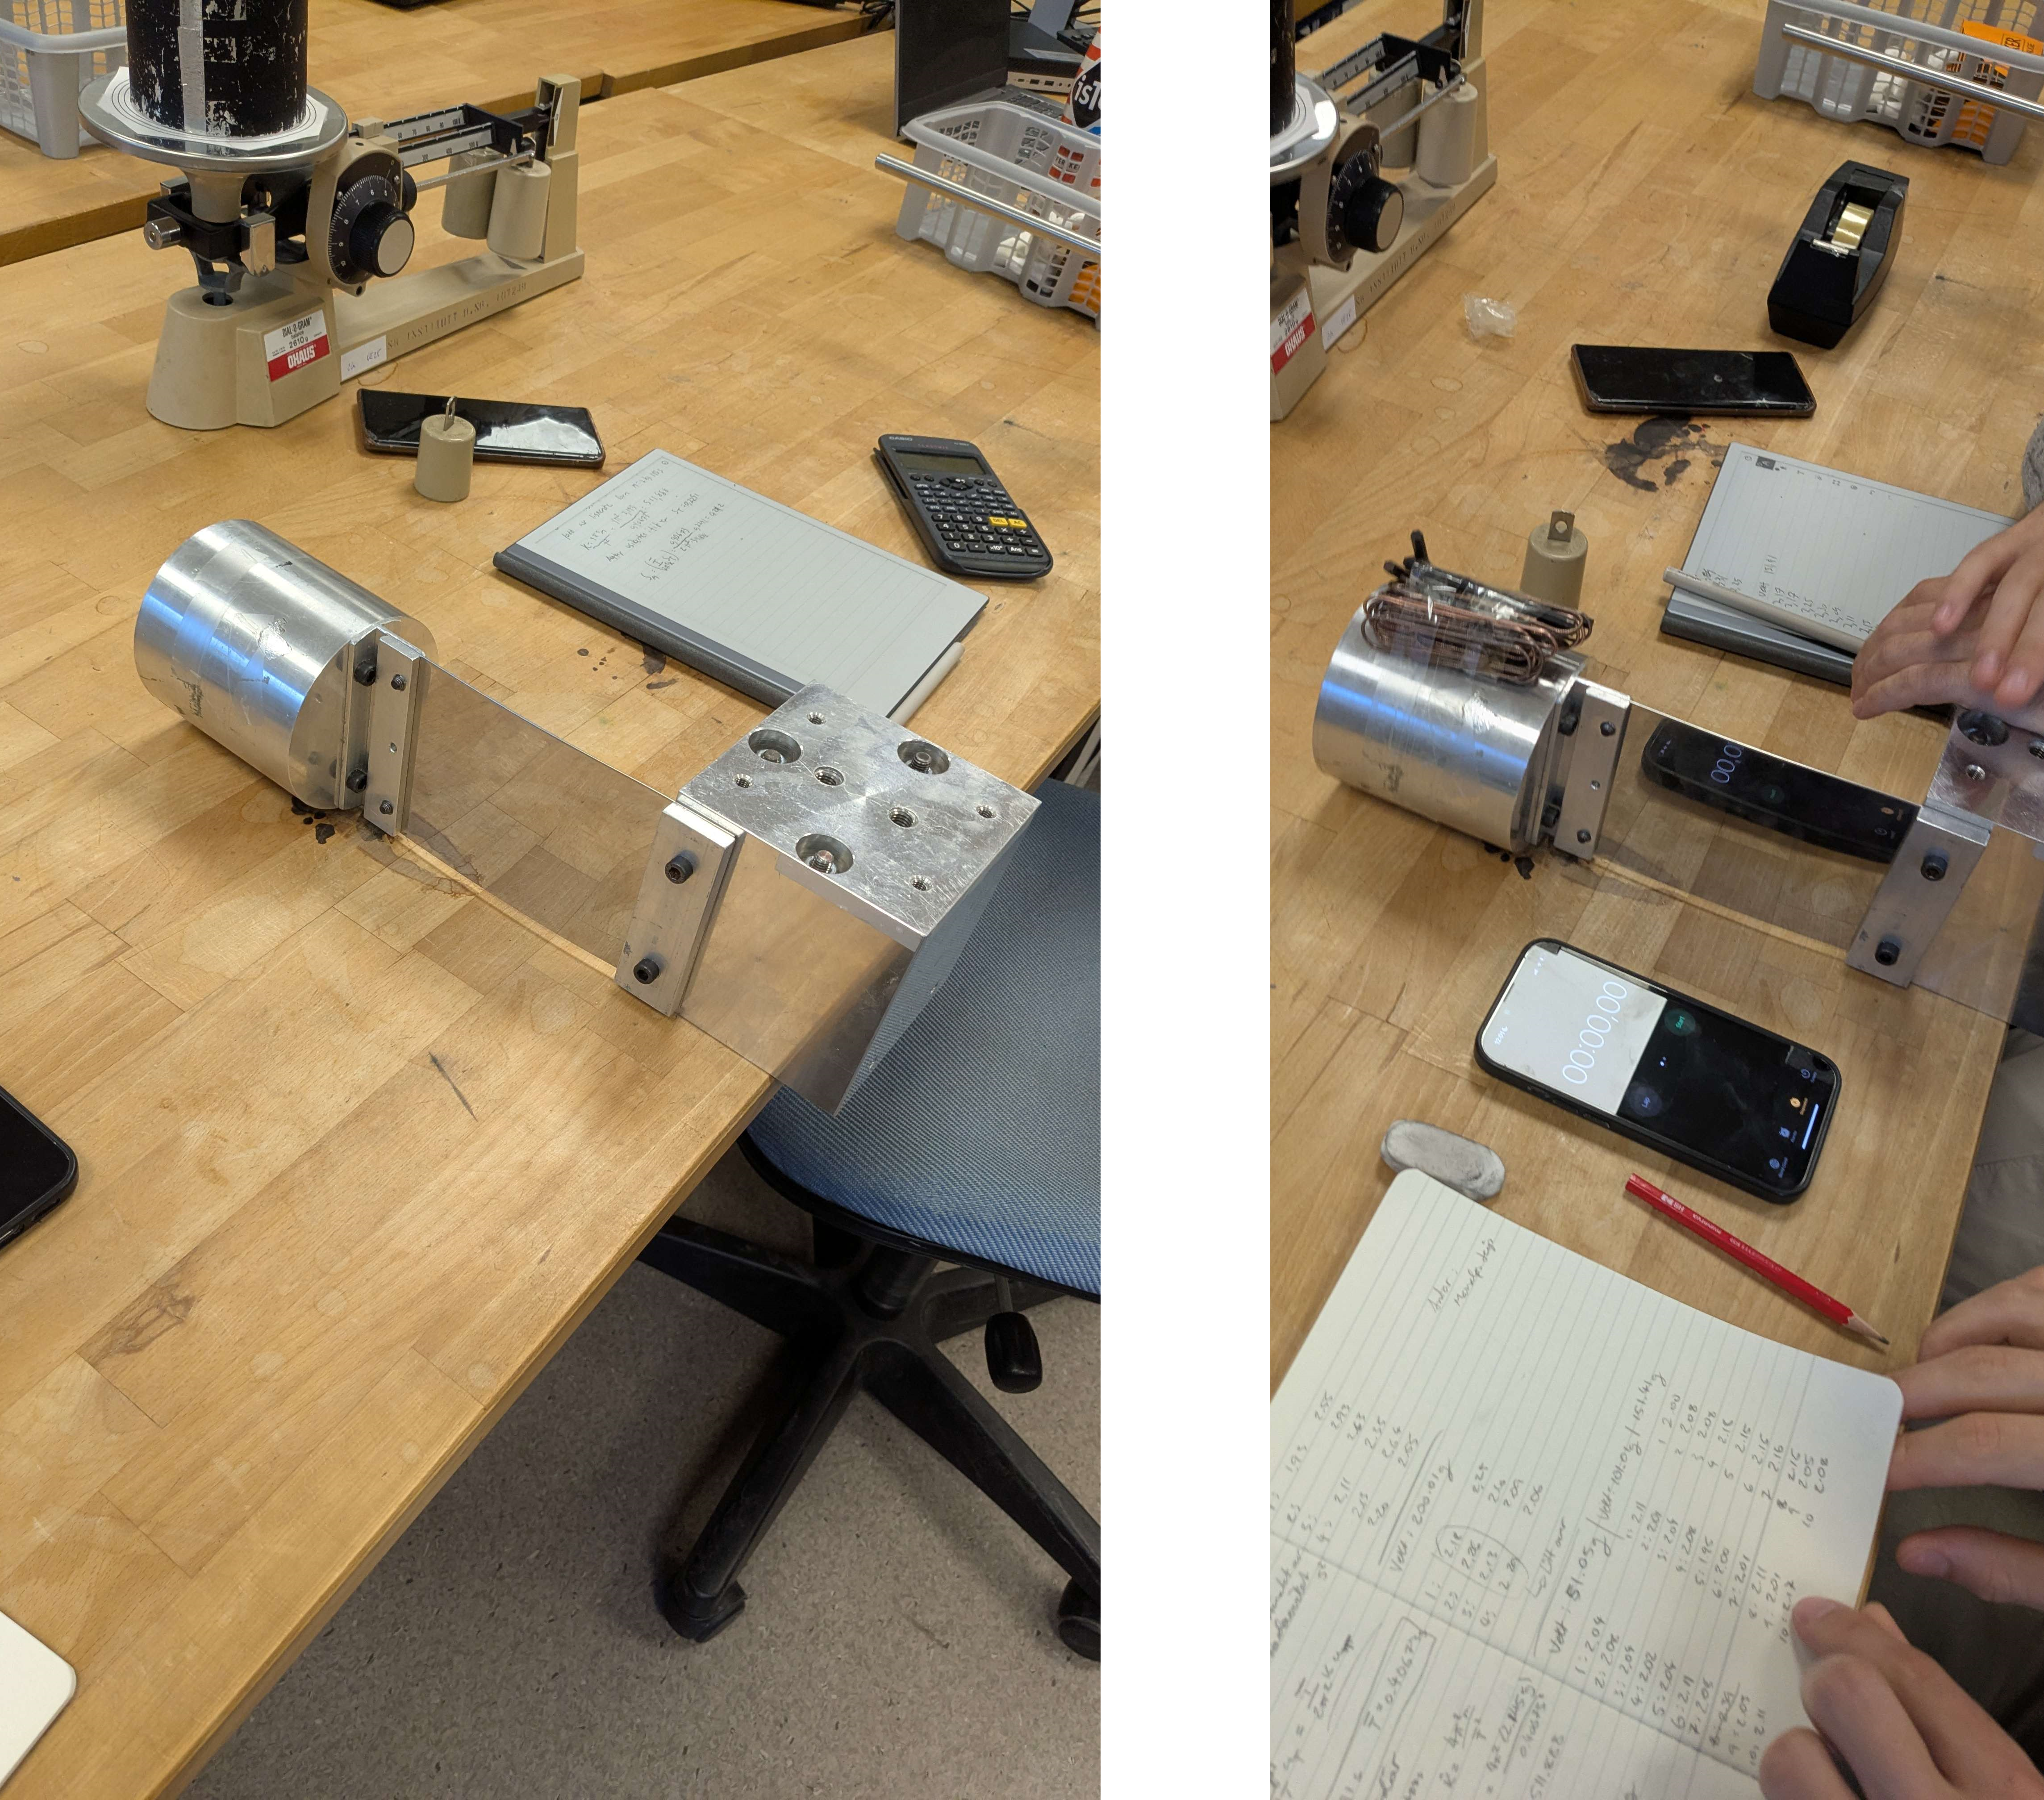
\includegraphics[scale = 0.07]{Figurer/Lab_Fig_e.png} 
\captionof{figure}{Vår harmoniske Oscillerator (Venstre), og samme oscillerator tilsatt en liten masse ca. lik $u_m$} \label{forsøk_e_fig}
\par \bigskip

Vi repeterte dette med masse ca. lik $2u_m$ og $3u_m$.\medskip

Til slutt plottet vi alle periodemålingene våre sammen i python.


\subsection{Resultater} \label{Resultater_2}

\subsubsection*{Forsøk d}
Vi fikk følgende kalibreringsmål:

\begin{center}
\begin{tabular}{  | c | c |}
    \hline
    Masse (g) & Lengde på deformasjon (mm)\\
    \hline
    0 & 6.16\\
    \hline
    1 & 6.16\\
    \hline
    10 & 6.14\\
    \hline
    100 & 5.93\\
    \hline
    110 & 5.92\\
    \hline
    500 & 4.97\\
    \hline
    510 & 4.96\\
    \hline
    600 & 4.68\\
    \hline
    610 & 4.67\\
    \hline
    1000 & 3.78\\
    \hline
    1010 & 3.76\\
    \hline
    1100 & 3.555 ($\pm 0.005$)\\
    \hline
    1110 & 3.53\\
    \hline
    1500 & 2.69\\
    \hline
    1510 & 2.665 ($\pm 0.005$)\\
    \hline
    1600 & 2.47\\
    \hline
    1610 & 2.455 ($\pm 0.005$)\\
    \hline
    2000 & 1.62\\
    \hline
    2100 & 1.40\\
    \hline
\end{tabular}
\captionof{table}{Lengden lest av måleuret for forskjellige kombinasjoner av kalibreringsloddene}
\end{center}

Vi tilpasset en lineær regresjonsmodell til disse målene (se vedlegg \ref{Kalibreringskurve.py} for kode), og fikk følgende graf og utrykk:

\begin{center}
\includegraphics[scale=0.7]{Figurer/Lab_2_regresjon.png}
\end{center}

\begin{align*}
    m(l) &= (2677.847483) + (-437.310226)\cdot l 
\end{align*}
\captionof{figure}{Lineær regresjonsmodell og korresponderende funksjonsutrykk.}
\bigskip

Når vi la aluminiumsloddet i kurven, leste vi av $1.27$ mm på måleuret. Dersom vi setter dette inn i funksjonen vi fant ved regresjonen, får vi at loddet har massen 2122.5 g. Så plottet vi residualer for denne regresjonsmodellen:

\begin{center}
\includegraphics[scale=0.7]{Figurer/Lab_2_Residualer.png}
\end{center}

Vi ser at residualene følger en kurve, der de korteste og lengste lengdene gir store positive avvik, mens lengdene mot midten gir store negative avvik.\medskip

Vi fikk følgende plott for regresjonsmodellens prediksjonsintervall:

\begin{center}
\includegraphics[scale=0.7]{Figurer/Lab_2_regresjon_prediksjon.png}
\end{center}

Programmet ga oss også usikkerhetene for store og små masser:
\begin{center}
\begin{tabular}{  | c | c |}
    \hline
    $u_{\text{små}}$ & 95.8\\
    \hline
    $u_{\text{store}}$ & 98.4\\
    \hline
\end{tabular}
\captionof{table}{Usikkerhetene for små og store masser (i gram)}
\end{center}

Vi kan da altså ikke måle masser under 95.8 gram.

Programmet ga oss også det dynamiske området, som var 1.34.

\subsubsection*{Forsøk e}

Mål for pendelens periodetider ligger vedlagt som vedlegg \ref{Perioder.txt}. Vårt mål av aluminumsloddet ble 2145g. Programmet lagt ved som \ref{Perioder.py} estimerte snittet av disse periodene, samt standardavviket. Programmet ga oss også standardfeil for disse målingene.

\begin{center}
\begin{tabular}{  | c | c |}
    \hline
    $\overline{t}$ & 0.406\\
    \hline
    $s_t$ & 0.0230\\
    \hline
    $SEM(t)$ & 0.00488\\
    \hline
\end{tabular}
\captionof{table}{Snitt, standardavvik, og standardfeil for pendelens periodetider (i sekunder).}
\end{center}

Så snur vi på formel \ref{periodformula} for å estimere k, ved hjelp av snitt-tiden og massen vi målte fra aluminiumsloddet. Dette gir oss:

\begin{align*}
    k &= \frac{4m\pi^2}{\overline{t}^2}\\
      &= \frac{4\cdot 2.145 \cdot \pi^2}{0.406^2} \; \text{kg/$s^2$}\\
      &= 513 \; \text{kg/$s^2$}
\end{align*}

Ved hjelp av formel \ref{gu} (og formel \ref{periodformula}) kan vi finne et uttrykk for usikkerheten i massen:

\begin{align*}
    u_m &= \frac{\overline{t}\cdot k \cdot SEM(t)}{2\cdot\pi^2}\\
    &= \frac{0.406 \cdot 513 \cdot 0.00488}{2\cdot \pi^2}\\
    &= 0.0515 \; \text{kg}\\
    &= 51.5 \; \text{g}
\end{align*}

Mål for periodetidene med $u_m, 2u_m$ og $3u_m$ tilsatt ligger også i vedlegg \ref{Perioder.txt}.
Disse periodetidene, plottet sammen med de originale periodetidene, ser slik ut:

\begin{center}

\includegraphics[scale = 0.45]{Figurer/Lab_2_Masse_Mot_Periode.png}
\includegraphics[scale = 0.45]{Figurer/Lab_2_Masse_Mot_Periode2.png}

\captionof{figure}{Plott av periodetid mot masse, sammen med snittet for hver masse. Her plottet med tid (venstre) og $\text{tid}^2$ (høyre).}
\label{MassePeriode}
    
\end{center}

\subsection{Diskusjon}

\subsubsection*{Forsøk d}

Vi så allerede ved andre mål at vekten ikke kunne måle masseforskjeller under 1g, og valgte dermed ikke å måle så små masseforskjeller. Vi valgte også ikke å måle høyere masser enn 2100, og når vi så brukte regresjonsmodellen vår til å finne massen til aluminiumsloddet, fant vi ut at aluminiumsloddet hadde høyere masse enn det vi målte med kalibreringsloddene. Vi har altså at aluminumsloddets masse er utenfor området vi har modellert, og vi kan dermed ikke være veldig sikre på tallet. \smallskip

Selv om vi ikke kan være veldig sikre på tallet, målte vi vekten til aluminiumsloddet for forsøk e, og vet dermed at vår estimerte masse er ganske nærme.\smallskip

Vi valgte å plotte masse mot lengde, som ga oss en omvendt proporsjonalitet mellom dem, men det hadde vært mer hensiktsmessig å ha differansen mellom lengden lest av måleuret uten masse og lengden lest av måleuret med masse på x-aksen. Denne differansen ville gått opp med massen, og vi hadde dermed fått en direkte proporsjonalitet i stedet. Dersom vi skulle gjennomført forsøket igjen, ville vi sannsynligvis gjort dette.\smallskip

Fra residualplottet kunne vi se et systematisk avvik, både mot midten av grafen og i endene. Dette kan selvsagt bety at vi kalibrerte feil, men mer sannsynlig er det noe feil i antakelsen vår om at massen og lengden er proporsjonale. \smallskip

Prediksjonsintervallet ga oss usikkerhetene i små og store masser, og disse usikkerhetene er relativt store. For små masser har vi også målt forskjeller på under 95.8g, som betyr at disse usikkerhetene ikke er helt riktige. Hadde vi hatt tid, hadde vi sjekket dette for store masser også. \smallskip

Til slutt i eksperimentet skulle vi måle aluminiumsloddet igjen sammen med en liten masse lik usikkerheten. På grunn av dårlig tid fikk vi ikke gjort dette.

\subsubsection*{Forsøk e}

Vi hadde ikke mulighet til å måle en og en periodetid, pendelen svingte fortere enn vi klarte å reagere. Dette er grunnen til at vi valgte å måle fem og fem svingninger, og så dele på fem etterpå. 
Aluminiumsloddet vi brukte til å anslå pendelens masse, var ikke det samme som loddet festet til pendelen. Dette introduserer selvsagt en usikkerhet, men vi valgte å neglisjere denne. \smallskip

Når vi fant konstanten $k$, antok vi at denne konstanten var idealistisk, altså at den riktig, og ikke endrer seg. Dette er den eneste måten vi kan bruke den samme formelen for å finne usikkerheten i massen. \smallskip

På plottet av periodetid mot masse, kan vi se at snittet av tidene vokser når massen vokser, i hvert fall for de to første masseøkningene. Dette tyder mot at vi kan bruke en pendel til å måle endringer i masse, men også kanskje at våre mål er for unøyaktige til å gjøre dette ordentlig. Vi begynte å få dårlig tid mot slutten av dette eksperimentet, som kan forklare dette.